\documentclass[cjk,dvipdfmx,10pt,compress,fragile%
hyperref={bookmarks=true,bookmarksnumbered=true,bookmarksopen=false,%
colorlinks=false,%
pdftitle={第 134 回 関西 Debian 勉強会},%
pdfauthor={小林},%
%pdfinstitute={関西 Debian 勉強会},%
pdfsubject={資料},%
}]{beamer}

\title{自作キーボード温泉に日帰り入浴してみた話}
\author[Katsuki Kobayashi]{{\large\bf Katsuki Kobayashi}}
\institute[Debian JP]{{\normalsize\tt 関西 Debian 勉強会}}
\date{{\small 2019年 11月 24日 (日)}}

\usepackage{graphicx}
\usepackage{moreverb}
\usepackage{ulem}
\usepackage[varg]{txfonts}
\usepackage{tabularx}
\usepackage{fancybox}
\usepackage{fancyvrb}
\usepackage{float}
\usepackage{multicol}
\usepackage{minijs}
\usepackage{amsmath}
\usepackage{amssymb}
\usepackage{newtxtext}
\usepackage{listings}
\usepackage{xcolor}
\usepackage{hyperref}
\AtBeginDvi{\special{pdf:tounicode EUC-UCS2}}
\usetheme{KansaiDebian}
\def\museincludegraphics{%
  \begingroup
  \catcode`\|=0
  \catcode`\\=12
  \catcode`\#=12
  \includegraphics[width=0.9\textwidth]}
%\renewcommand{\familydefault}{\sfdefault}
%\renewcommand{\kanjifamilydefault}{\sfdefault}
%
\newenvironment{commandline}%
{\VerbatimEnvironment
  \begin{Sbox}\begin{minipage}{0.9\hsize}\begin{fontsize}{8}{8} \color{white} \begin{BVerbatim}}%
{\end{BVerbatim}\end{fontsize}\end{minipage}\end{Sbox}
  \setlength{\fboxsep}{8pt}
% start on a new paragraph

\vspace{6pt}% skip before
\fcolorbox{white}{black}{\TheSbox}

\vspace{3pt}% skip after
}
%end of commandline

\begin{document}

\begin{frame}[fragile]
\titlepage
\end{frame}

\begin{frame}[fragile,t]{お詫び}
 \begin{itemize}
  \item Debian要素はあんまりないです
 \end{itemize}
\end{frame}

\takahashi[40]{みなさん}
\takahashi[40]{肩や腰は\\大丈夫ですか?}
\takahashi[40]{私は駄目です}

\begin{frame}[fragile,t]{自作キーボードへの動機(1/4)}
 \begin{itemize}
  \item 会社にて腰痛が酷くて、対策しても効果がない
	\begin{itemize}
	 \item 整骨院に通う
	 \item ジムで筋トレする
	\end{itemize}
  \item 特に、ここ数年酷い
	\pause
  \item 心当たり
 \end{itemize}
\begin{center}
 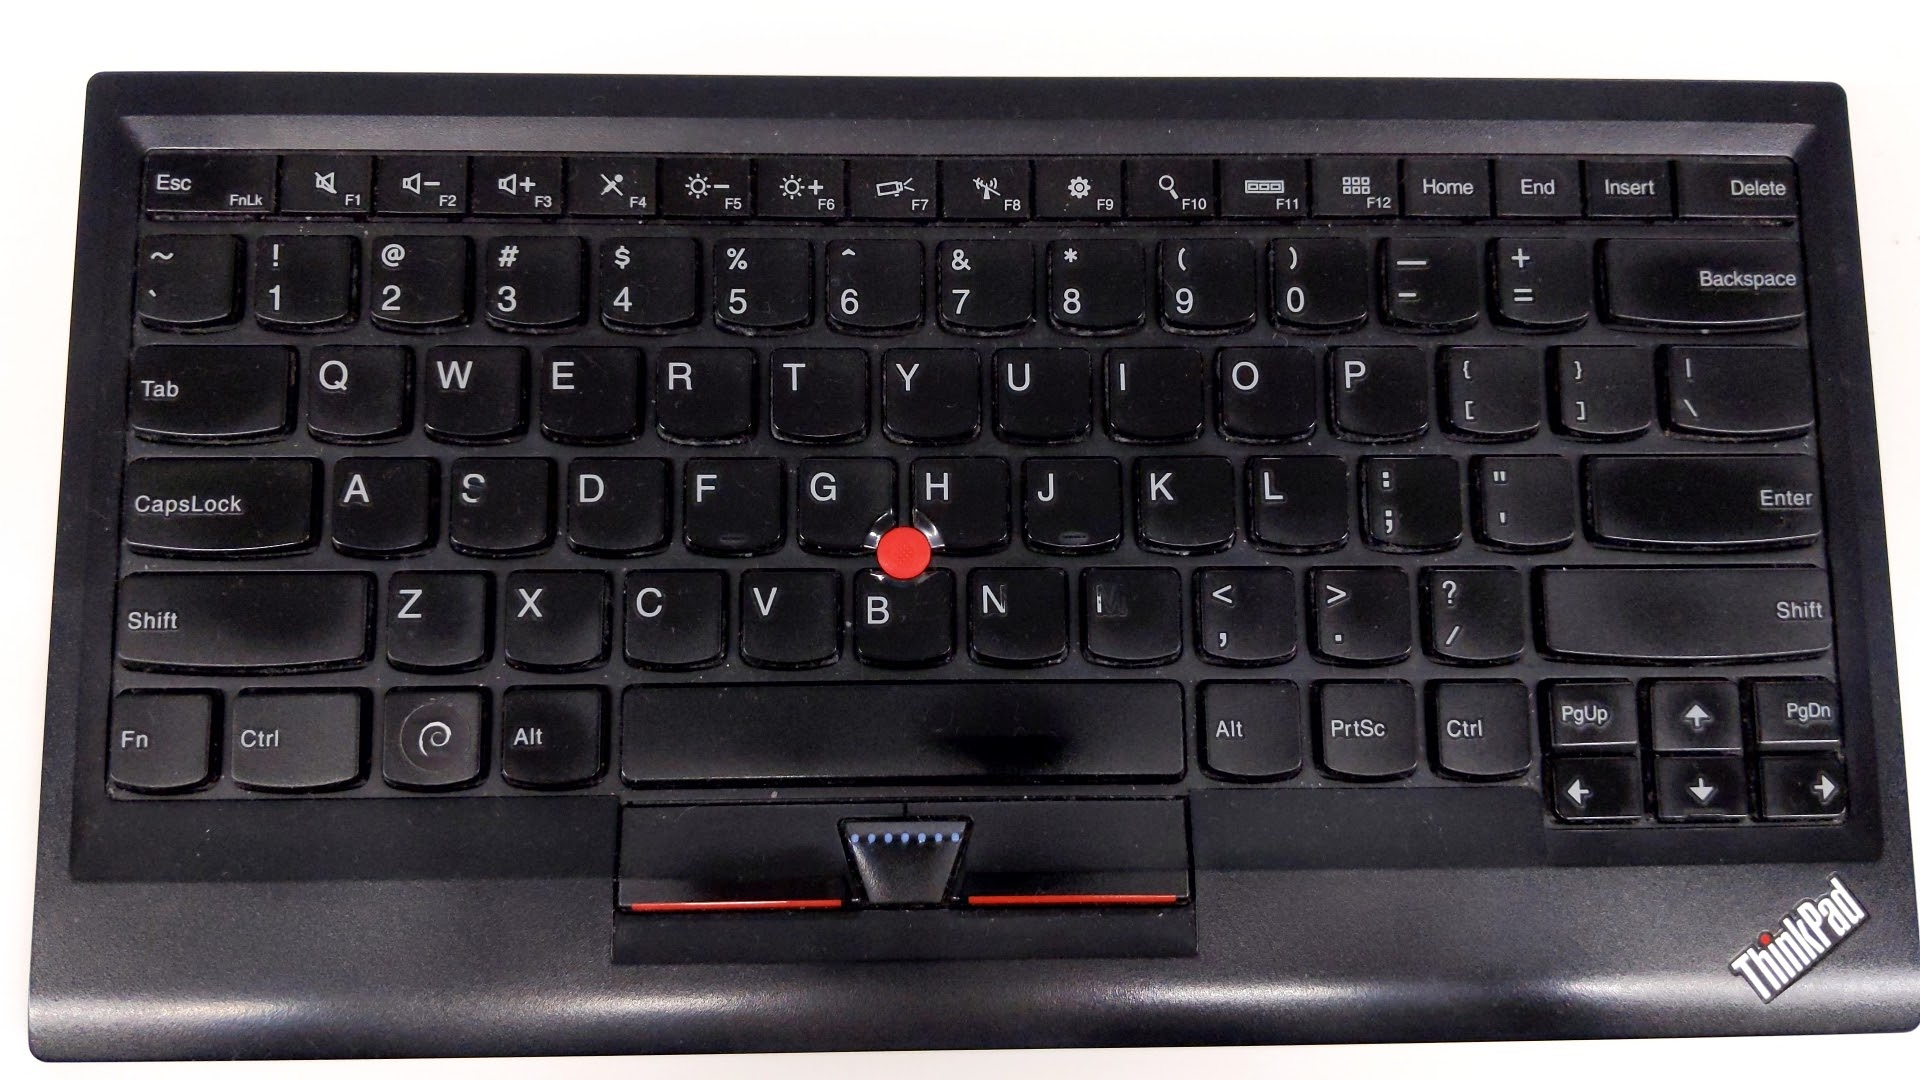
\includegraphics[keepaspectratio,height=4cm]{./img/thinkpad_kb.jpg}
\end{center}
\end{frame}

\begin{frame}[fragile,t]{自作キーボードへの動機(2/4)}
 \begin{itemize}
  \item ThinkPadキーボード
	\begin{itemize}
	 \item ThinkPadを使い始めて約4年
	 \item トラックポイントの良さに気付いて会社でもThinkPadキーボードに
	       \begin{itemize}
		\item WindowsではLinuxほど恩恵には預かれないけど
	       \end{itemize}
	 \item トラックポイントが悪いのかと思い、ここ数ヶ月はマウスを使用
	       \begin{itemize}
		\item しかし改善せず……
	       \end{itemize}
	\end{itemize}
	\pause
  \item 分割型キーボード
	\begin{itemize}
	 \item まぁ、肩凝りには効きそう
	 \item しかし、腰に効くのか想像できない
	\end{itemize}
 \end{itemize}
\end{frame}

\begin{frame}[fragile,t]{自作キーボードへの動機(3/4)}
 \begin{itemize}
  \item \href{https://ultimatehackingkeyboard.com/}{Ultimate Hacking Keyboard}なるものをみつける
	\begin{itemize}
	 \item トラックポイントが付く!!
	       \begin{itemize}
		\item しかし場所がおかしい
		\item トラックボールやタッチパッドも付けられる
	       \end{itemize}
	 \item 軸は変更できる
	       \begin{itemize}
		\item 軸については後ほど……
	       \end{itemize}
	 \item ファームもカスタマイズできる
	 \item でもお値段的に
	       \begin{itemize}
		\item 最小構成でも275ドル
		\item トラックポイントつけたらいレストアームつけると4万円越え
	       \end{itemize}
	\end{itemize}
 \end{itemize}
\end{frame}

\begin{frame}[fragile,t]{自作キーボードへの動機(4/4)}
 \begin{itemize}
  \item 沼の住人からお声かけいただく
	\begin{itemize}
	 \item \url{https://twitter.com/rarewin/status/1163656414184689665}
	\end{itemize}
  \item \href{https://mechanicalkeyboards.com/shop/index.php?l=product_detail&p=3532}{Tex Yoda II}
	\begin{itemize}
	 \item 分割されてたら求めていた感じだった
	\end{itemize}
  \item 自作キーボードにトラックポイントを付けている人は一定数いるらしい
	\begin{itemize}
	 \item \href{https://www.google.com/search?client=firefox-b-e&q=%E3%83%88%E3%83%A9%E3%83%83%E3%82%AF%E3%83%9D%E3%82%A4%E3%83%B3%E3%83%88+%E8%87%AA%E4%BD%9C%E3%82%AD%E3%83%BC%E3%83%9C%E3%83%BC%E3%83%89}{Google検索: トラックポイント 自作キーボード}
	\end{itemize}
  \item そんなこんなで、自作へと心が……
 \end{itemize}
\end{frame}

\end{document}